\documentclass[14pt]{beamer} %Makes presentation
%\documentclass[handout]{beamer} %Makes Handouts
\usetheme{Singapore} %Gray with fade at top
\useoutertheme[subsection=false]{miniframes} %Supppress subsection in header
\useinnertheme{rectangles} %Itemize/Enumerate boxes
\usecolortheme{seagull} %Color theme
\usecolortheme{rose} %Inner color theme

\definecolor{light-gray}{gray}{0.75}
\definecolor{dark-gray}{gray}{0.55}
\setbeamercolor{item}{fg=light-gray}
\setbeamercolor{enumerate item}{fg=dark-gray}

\setbeamertemplate{navigation symbols}{}
%\setbeamertemplate{mini frames}[default]
\setbeamercovered{dynamics}
\setbeamerfont*{title}{size=\Large,series=\bfseries}

%\setbeameroption{notes on second screen} %Dual-Screen Notes
%\setbeameroption{show only notes} %Notes Output

\setbeamertemplate{frametitle}{\vspace{.5em}\bfseries\insertframetitle}
\newcommand{\heading}[1]{\noindent \textbf{#1}\\ \vspace{1em}}

\usepackage{bbding,color,multirow,times,ccaption,tabularx,graphicx,verbatim,booktabs,fixltx2e}
\usepackage{colortbl} %Table overlays
\usepackage[english]{babel}
\usepackage[latin1]{inputenc}
\usepackage[T1]{fontenc}
\usepackage{lmodern}

%\author[]{Thomas J. Leeper}
\institute[]{
  \inst{}%
  Department of Government\\London School of Economics and Political Science
}

\usepackage{tikz}
\usetikzlibrary{shapes,arrows,positioning}

\title{Concepts\\{\small ``I'll know it when I see it''}}

% Before we can study something we need to know what that ``something'' is. This is concept definition. How do we define concepts and how do we separate different concepts from one another?

\date[]{}

\begin{document}

\frame{\titlepage}

\frame{

\frametitle{Goal for Today}

\large
\begin{center}
Develop the ability to formally and precisely \textit{define} ``concepts'' using two common approaches to concept definition, and beginning thinking about how to assess the quality of competing definitions
\end{center}

}


\frame{\tableofcontents}

\section{Concepts}
\frame{\tableofcontents[currentsection]}

\frame{
\frametitle{Concepts}

\begin{itemize}\itemsep0.5em
\item Definition: The words and ideas that we use to describe the world

\item<2-> Why do we care?
	\begin{itemize}\itemsep0.5em
	\item<3-> We cannot theorize a phenomenon until we know what it is
	\item<4-> We cannot agree on or debate measure of things until we share a definition of what we're trying to measure
	\item<5-> Problem Set 1 is due soon
	\end{itemize}

\end{itemize}
}

% we can look to literature or we can develop our own concepts, but as we'll talk about in a few minutes we don't want to create new concepts unless they are useful and meaningful

\frame{

Concepts are useful because they distinguish things from other things.

\vspace{1em}

In particular, they:

\begin{enumerate}
\item Resolve ambiguity
% label connected to multiple meanings
% meaning connected to multiple labels

\item Avoid vagueness % lack of a good definition
\end{enumerate}

\vspace{0.5em}
This allows us to talk precisely about phenomena without confusion or cross-talk.
}

% For example, if we want to build an understanding of the concept ``democracy'' (such as its effects on economic outcomes, or the processes that cause democracies to form) then we need to be clear about what we mean by democracy. We need to distinguish it from other concepts that might be related but that are different (autocracy, oligarchy, anarchy, state, nation-state, liberal society, etc.).


\begin{frame}[fragile]
\frametitle{{\large Ogden \& Richard's Triangle\footnote{Richards, I.A., and Ogden, C.K. 1923 \textit{The Meaning of Meaning}.}}}

\begin{tikzpicture}
\node[align=center, text width=3.5cm] at (0,0) (label) {Label};
\node[align=center, text width=3.5cm] at (3,3) (meaning) {Meaning};
\node[align=center, text width=3.5cm] at (6,0) (cases) {Cases};

\draw[<->,very thick] (label) to (meaning);
\draw[<->,very thick] (cases) to (meaning);

\end{tikzpicture}
% meaning (set of ideas we associate with a concept; the essential constitutive elements)
% label (word used to designate a concept)
% cases (entities that are instances or cases of a concept)

\end{frame}


\frame{
\frametitle{Quick Brainstorm}

\only<1>{\vskip20pt}

\large
\begin{center}
What are some important political science concepts?
\end{center}

\only<2->{
\vspace{-0.5em}
\footnotesize
\begin{columns}
\begin{column}{0.29\textwidth}
   \begin{itemize}
   \item Democracy
   \item Inequality
   \item Populism
   \item Extremist
   \item Nation
   \end{itemize}
\end{column}
\begin{column}{0.29\textwidth}  %%<--- here
   \begin{itemize}
   \item Opinion
   \item Values
   \item Ideology
   \item War
   \item Liberty
   \end{itemize}
\end{column}
\begin{column}{0.38\textwidth}  %%<--- here
   \begin{itemize}
   \item Political party
   \item Immigrant
   \item Social movement
   \item Authoritarianism
   \item Development
   \end{itemize}
\end{column}
\end{columns}
}
}





\frame{
\frametitle{{\normalsize Approaches to Concept Definition}}

Two common approaches:\\

\vspace{1em}

\begin{enumerate}\itemsep1em
\item Classical Approach
\item Family Resemblance
\end{enumerate}

\vspace{1em}
There are other ways to define concepts but these are the most important.

}

\frame{
\frametitle{Simple Boolean Logic}

\begin{itemize}\itemsep1em
\item \textbf{AND}: necessity
	\begin{itemize}
	\item Represented by $\land$
	\item For attributes \textit{required} for a given instance be considered a member of the concept's set
	\end{itemize}
\item \textbf{OR}: sufficiency
	\begin{itemize}
	\item Represented by $\lor$
	\item For attributes \textit{optional} for a given instance be considered a member of the concept's set
	\end{itemize}
\end{itemize}

}


% Gerring distinguishes between minimal (classical approach); maximal (ideal types; Think Dahl and democracy as an ideal type); cumulative (more or less of a concept)
% the last of these will be particularly helpful when we start thinking about operationalization or measurement next week


\section[Classical Approach]{Concepts: Classical Approach}
\frame{\tableofcontents[currentsection]}


\frame{
\frametitle{Classical Approach}


\begin{itemize}\itemsep0.5em
\item Specify a set of ``constitutive dimensions'' that \textit{are} the concept
	\begin{itemize}
	\item Fundamental characteristics of the concept
	\item Not causes or effects
	\item Not measures of the concept
	\end{itemize}
\item<2-> Dimensions are \textit{individually necessary} and \textit{jointly sufficient} for a case to be a member of the concept set

\end{itemize}
}


\frame{
\frametitle{{\large Dahl's Definition of Democracy}}

\small 

\begin{itemize}\itemsep0.5em
\item Two dimensions
	\begin{itemize}
	\item<2-> Liberalization (Public contestation)
	\item<2-> Inclusiveness (Participation)
	\end{itemize}
\item Both necessary and jointly sufficient
\item<3-> Without liberalization: ``inclusive hegemony''
\item<4-> Without inclusiveness: ``competitive oligarchy''
\end{itemize}

}


\frame{\huge\vskip20pt\textbf{Questions?}}

\frame[label=chairexample]{

\title{Example}

Define the concept of ``\hyperlink{chairs}{chair}''

\begin{center}
\includegraphics[height=0.7\textheight]{images/chair}
\end{center}

{\tiny \href{https://commons.wikimedia.org/wiki/File:Chair_5709.jpg}{Image Source: Wikimedia} by \href{https://commons.wikimedia.org/wiki/User:Dori}{User:Dori}}
}


\section[Family Resemblance]{Concepts: Family Resemblance}
\frame{\tableofcontents[currentsection]}

\frame{
\frametitle{Family Resemblance}

\begin{itemize}\itemsep0.5em
\item Classical approach focuses on \textit{necessity}
\item Some concepts have no necessary elements but are still meaningful % Game
\item<2-> We might also think about elements that are individually or jointly \textit{sufficient} to establish membership
\end{itemize}
}

\frame{
\frametitle{Complex Boolean Logic}

\small

\begin{itemize}\itemsep0.5em

\item Jointly necessary and sufficient:\\
\hspace{1em} {\footnotesize $\text{Rule of Law} \land \text{Equality}$}

\item<2-> Jointly necessary w/ insufficient attributes\\
\hspace{1em} {\footnotesize $\text{Rule of Law} \land (\text{Equality} \lor \text{Elections}) $}

\item<3-> Simple family resemblance logic:\\
\hspace{1em} {\footnotesize $(\text{Equality} \lor \text{Elections})$}

\item<4-> Complex family resemblance logic:\\
\hspace{1em} {\footnotesize $(\text{Rule of Law} \land \text{Participation}) \lor (\text{Equality} \land \text{Elections}) $}

\end{itemize}

}

\begin{frame}[fragile]
\large
\begin{center}
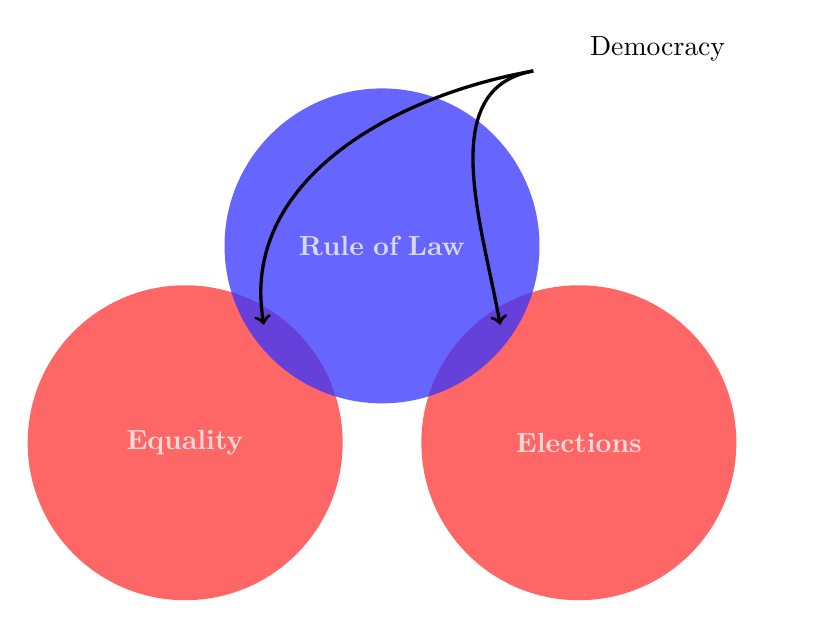
\begin{tikzpicture}
    \fill[red!80,opacity=0.75] (0,0) circle (2cm) 
            node[text=white, align=center, text width=3cm] {\textbf{Equality}};
    \fill[red!80,opacity=0.75] (5,0) circle (2cm) 
        node[text=white, align=center, text width=3cm] {\textbf{Elections}};
    \fill[blue!80,opacity=0.75] (2.5,2.5) circle (2cm) 
            node[text=white, align=center, text width=3cm] {\textbf{Rule of Law}};
    \node[align=center, text width=3.5cm] at (6,5) (c) {Democracy};
    \draw[->,very thick] (c) to [out = 190, in = 100, looseness = 1] (4,1.5);
    \draw[->,very thick] (c) to [out = 190, in = 100, looseness = 1] (1,1.5);
\end{tikzpicture}
\end{center}
\end{frame}


\frame{\huge\vskip20pt\textbf{Questions?}}


\begin{frame}[label=game, fragile]

\frametitle{Example: Define ``game''}

\vspace{-2.2em}

\begin{center}
\resizebox{\textwidth}{0.75\textheight}{%
\begin{tikzpicture}
  \node (img1) {\includegraphics[height=3cm]{images/rugby}};
  \node (img2) [below right=-1cm and -1.5cm of img1] {\includegraphics[height=3cm]{images/chess}};
  \node (img3) [below=-0.5cm of img1] {\includegraphics[height=3cm]{images/gameboy}};
  \node (img4) [above right=-2.5cm and -0.25cm of img1]  {\includegraphics[height=3cm]{images/cribbage}};
  \node (img5) [below right=0.5cm and -2cm of img4]  {\includegraphics[height=3cm]{images/tugofwar}};
  \node (img6) [above right=-1cm and 0.5cm of img2]  {\includegraphics[height=3cm]{images/cards}};
\end{tikzpicture}
}
\end{center}

\vspace{-1em}

\hyperlink{gamesources}{\beamergotobutton{Image Sources}}

\end{frame}







\section{Evaluating Concept Definitions}
\frame{\tableofcontents[currentsection]}

\frame{

\frametitle{Other Approaches}

\begin{itemize}\itemsep0.5em
\item Two most common ways to think about concepts
	\begin{itemize}
	\item Classical approach (emph. necessity)
	\item Family resemblance (emph. sufficiency)
	\end{itemize}
\item These are useful when defining \textit{things}
\item<2-> Other approaches might be useful when defining \textit{processes}
	\begin{itemize}
	\item Mansbridge's definitions of \textit{representation}
	\item First, Second, and Third \textit{faces of power}
	\item In LT: notions of causality
	\end{itemize}
\end{itemize}

}


\begin{frame}[fragile]

\frametitle{Trade-offs in Definitions}

\vspace{-2em}

\begin{center}
\begin{tikzpicture}
	% x-axis
    \draw[->] (0,0) node[below] (origin) {} -- (5,0) node[right] (xaxis) {};
    \node[below] at (2.5,-0.75) {\small Intension (More attributes)};
	\node[below] at (0.5,0) {\footnotesize Low};
	\node[below] at (5,0) {\footnotesize High};
	
	% y-axis
    \draw[->] (origin) -- (0,5) node[left] (yaxis) {};
	\node[left, text width=5cm, align=center] at (0,2.5) {\small Extension\\(More cases)};
	\node[left] at (0,0.5) {\footnotesize Low};
	\node[left] at (0,5) {\footnotesize High};

    \draw<2,4>[<->, dashed] (0.5,4.5) -- (4.5,0.5);
    \node<2,4>[rotate=-45] at (4,1.25) {\tiny Necessary};
    
    \draw<3-4>[<->, dashed] (0.5,0.5) -- (4.5,4.5);
    \node<3-4>[above, rotate=45] at (4,4) {\tiny Sufficient};

\end{tikzpicture}
\end{center}
\end{frame}

% Need to balance specificity against abstraction/generality
% In classical approach, intension and extension are inversely related (Gerring Fig. 5.1)
% In family resemblance approach, intension and extension are positively related
% If we increase necessary attributes, we have fewer cases of that concept and it is more specific
% If we increase sufficient attributes, we have more cases of that concept and it is more general



\frame{
\frametitle{Gerring's Criteria}

\begin{enumerate}
\item Resonance
\item Domain/scope % ladder of generality
\item Consistency
\item Fecundity
\item Differentiation
\item Causal utility
\item Operationalization (next week)
\end{enumerate}
}

% divide these up and have someone present each one


% Resonance: Is the concept intuitive? Avoid neologism (Gerring p.118); we don't need new terms for the sake of having new terms

% Domain: The contexts in which this concept resonates and applies. Example: "vouchers". What does this mean? This has a clear meaning in the United States, in debates about education policy, but that is a narrow domain. Contrast this with democracy or terrorism, which are concepts with broad domains.

% Consistency: We can change the definition of a concept by adding, removing, or modifying attributes; Contrast with "slippage" or "stretching"

% Fecundity: Fertility or fruitfulness; Neologisms are prone to lacking fecundity

% Differentiation: How does this concept contrast or help create distinctions between existing sets of phenomena? Example: *Opinion* is a summary evaluation of a particular object; *Value* is a belief about a desired end-state of the world

% Causal Utility: Concept has to be useful for making a causal argument; this may require a concept to be more specific or have higher intensity than we would prefer because we need to *use* the concept

% Operationalization: concepts have to be measurable; we'll talk about this next week

\frame{\huge\vskip20pt\textbf{Questions?}}

\frame{

\frametitle{In Sum}

\begin{itemize}\itemsep0.5em
\item We need to know what we're talking about before we can study anything empirically
\item Concept vary in their usefulness and are often contestable
\item Many ways to define and evaluate the quality of concepts
\end{itemize}

}



\appendix
\frame{}

\frame[label=gamesources]{

\tiny

\begin{itemize}
\item Rugby: flickr user Paddy-K \url{https://commons.wikimedia.org/wiki/File:Jonny_Wilkinson_2009_08_england_training_2.jpg}
\item Chess: Wikimedia user MichaelMaggs \url{https://commons.wikimedia.org/wiki/File\%3AOpening_chess_position_from_black_side.jpg}
\item Gameboy: Public domain \url{https://commons.wikimedia.org/wiki/File\%3AGameboy.jpg}
\item Cribbage: Wikimedia user Aerion \url{https://commons.wikimedia.org/wiki/File:120-hole_cribbage_board.jpg}
\item Cards: Public domain \url{https://commons.wikimedia.org/wiki/File\%3AEuchre.jpg}
\item Tug of war: Wikimedia user Johnmoore6 \url{https://en.wikipedia.org/wiki/File:Irish_600kg_euro_chap_2009.JPG}
\end{itemize}

\hyperlink{game}{\beamergotobutton{Return to Images}}

}

\frame[label=chairsources]{

\tiny

\begin{itemize}
\item images/chair: Wikimedia user Dori \url{https://commons.wikimedia.org/wiki/File:Chair_5709.jpg}
\item images/throne: Wikimedia user Badseed  \url{https://commons.wikimedia.org/wiki/File:Ottoman_throne.jpg}
\item images/beanbag: Wikimedia user Pava  \url{https://commons.wikimedia.org/wiki/File:\%22_12_-_ITALY_-_Pouf_Tuffet_Sacco_di_Zanotta_red_armchair_Triennale_Design_Museum.jpg}
\item images/kneelingchair: Wikimedia user TonyTheTiger  \url{https://commons.wikimedia.org/wiki/File:Deluxe_kneeling_chair.jpg}
\item images/bench: Wikimedia user 4028mdk09  \url{https://commons.wikimedia.org/wiki/File:Holzbank_mit_schmiedeeisener_R\%C3\%BCckenlehne.JPG}
\item images/trainseat: Wikimedia user Lover Of Romance \url{https://commons.wikimedia.org/wiki/File:Green-Car\%27s_Seat_of_JR_215.JPG}
\item images/hermanmiller: Wikimedia user Luiscarlosrubino \url{https://commons.wikimedia.org/wiki/File:Mirra_Chair_by_Studio_7.5_-_Herman_Miller.jpg}
\item images/wc: Public Domain \url{https://commons.wikimedia.org/wiki/File:Wc1.jpg}
\item images/stool: Wikimedia user Chatsam \url{https://commons.wikimedia.org/wiki/File:Pied_d\%27\%C3\%A9l\%C3\%A9phant_marche_pied.jpg}

\end{itemize}

\hyperlink{chairs}{\beamergotobutton{Return to Images}}

}

\frame[label=chairs]{

\includegraphics[width=2.25cm]{images/chair}
\includegraphics[width=1.75cm]{images/throne}
\includegraphics[width=2.25cm]{images/hermanmiller}
\includegraphics[width=1.75cm]{images/wc}
\includegraphics[width=2.7cm]{images/beanbag}

\includegraphics[width=2.5cm]{images/stool}
\includegraphics[width=5cm]{images/bench}
\includegraphics[width=2.8cm]{images/trainseat}

\hyperlink{chairexample}{\beamergotobutton{Return to Slides}} \hyperlink{chairsources}{\beamergotobutton{Image Sources}}

}

\end{document}
